% !TEX encoding = UTF-8 Unicode
\RequirePackage{fix-cm}
\documentclass[a4paper,10pt,UTF8]{paper}
%\documentclass[a4paper,10pt,UTF8]{ctexart}

\usepackage[english]{babel}
\usepackage{fancyhdr,array,lastpage,amsmath,mathtools,enumitem,graphicx,multirow,tocbibind,longtable,makecell,varwidth,titlesec,bm,booktabs,comment,minted}
\usepackage{enumitem}
\usepackage{hyperref}
\hypersetup{hidelinks}




\usepackage[left=2.54cm,right=2.54cm,top=2.54cm,bottom=2.54cm]{geometry}
\usepackage[font=footnotesize,labelfont=bf]{caption}
\usepackage{tikz,flowchart}
\usepackage{ctex}
\usepackage{xeCJK}%中文字体
\usetikzlibrary{shapes,shapes.geometric,arrows,matrix,calc}
\usetikzlibrary{circuits.logic}

% \usetikzlibrary{circuits.logic.custom}
\usetikzlibrary{circuits.logic.IEC}
\usetikzlibrary{shadows}
\usepackage{listings}
\usepackage[Q=yes]{examplep}
\usepackage{fancyhdr}
\usepackage{alphalph}
\usepackage{indentfirst}

% \setCJKsansfont{黑体}
\setmainfont{PingFang SC}
\setCJKmainfont{PingFang SC}
\setCJKsansfont{PingFang SC}
\setmonofont{Monaco}

\newenvironment{sol}
  {\par\vspace{2mm}\noindent{\bf Solution}. }

\lstset{escapeinside=``, breaklines=true, frame=none, extendedchars=false, basicstyle=\ttfamily, showstringspaces=false}


\setlength{\parindent}{2em}
\setlength{\parskip}{1.5ex plus 0.5ex minus 0.2ex}
\linespread{1.1}

\bibliographystyle{plain}

\numberwithin{equation}{section}
\numberwithin{figure}{section}


\setcounter{secnumdepth}{3}
\setcounter{tocdepth}{3}

\title{华东师范大学计算机科学技术系上机实验报告}

\begin{document}
\pagestyle{fancy}
\chead{\small\color{gray}华东师范大学计算机科学技术系上机实验报告}
\lhead{}
\rhead{}
\makeatletter
\def\headrule{{\if@fancyplain\let\headrulewidth\plainheadrulewidth\fi%
\color{gray}\hrule\@height 0.2pt\@width\headwidth}
  \vspace{6mm}}
\makeatother

\newcommand{\HRule}{\rule{\linewidth}{1mm}}
\newcommand{\dai}{\textbf{Dais-CMX16$^+$}}

{\center {\huge \bfseries \LARGE{华东师范大学计算机科学技术系上机实验报告}} \\ [0.8cm]

\small{
  \begin{minipage}[t]{.32\linewidth}
    \textbf{课程名称:}嵌入式原理与实践\\
    \textbf{指导教师:}沈建华\\
    \textbf{上机实践名称:} UART+RTC\\
    \textbf{实践编号:}实验 10
  \end{minipage}
  \begin{minipage}[t]{.32\linewidth}
    \textbf{年级:}17 级\\
    \textbf{姓名:}朱桐\\
    \textbf{学号:}10175102111\\
    \textbf{组号:}A
  \end{minipage} 
  \begin{minipage}[t]{.32\linewidth}
    \textbf{上机实践成绩:} \\
    \textbf{创新实践成绩:} \\
    \textbf{上机实践日期:}2019/12/10\\
    \textbf{上机实践时间:}2 学时\\
  \end{minipage}
}
\HRule \\[0.5cm]
}

\definecolor{bg}{rgb}{0.95,0.95,0.95}
\newminted{asm}{bgcolor=bg}
\newminted{c}{bgcolor=bg}

\NewDocumentCommand{\cw}{v}{\texttt{\textcolor{black}{#1}}}

\section{实验目的}

\begin{enumerate}
    \item 了解UART通信协议,掌握UART基本结构并学会相关参数的配置
    \item 掌握RTC时钟的配置和定时中断。
\end{enumerate}

\section{实验设备}

\begin{enumerate}
  \item 软件Keil5
  \item MSP-EXP432P401R LaunchPad开发板
\end{enumerate}


\section{实验内容}

\begin{enumerate}
  \item 使用MSP432的UART模块实现数据的收发;
  \item 使用MSP432的RTC模块实现定时功能;
  \item 完成课堂练习:使用UART控制RGB灯。
\end{enumerate}

\section{实验原理}

XDS110-ET 板载调试探针:
XDS110-ET 提供了一种与主机之间的“反向通道”UART-over-USB 连接,MSP432 UART串口反向映射为虚拟串口,在设备管理器中可以查看。

从原理图 \ref{fig:1}, \ref{fig:2} 可以看到XDS110-ET 隔离块J101的TXD和RXD分别对应引脚P1.2和P1.3。

\begin{figure}[h]
  \centering
  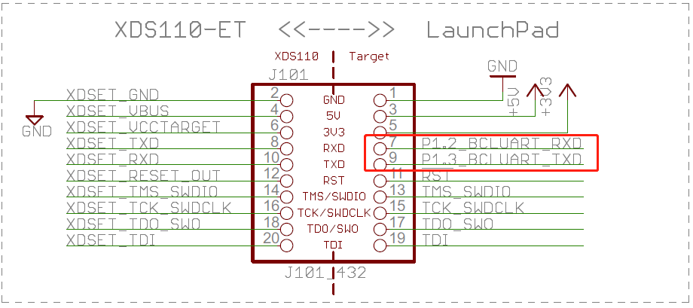
\includegraphics[width=0.5\textwidth]{img/1.PNG}
  \caption{相关原理图}
  \label{fig:1}
\end{figure}

\begin{figure}[h]
  \centering
  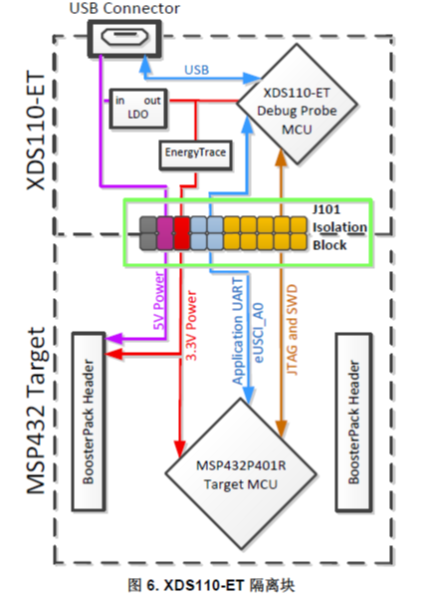
\includegraphics[width=0.5\textwidth]{img/2.PNG}
  \caption{相关原理图}
  \label{fig:2}
\end{figure}



\subsection{URAT简介}

UART(Universal Asynchronous Receiver/Transmitter)即“通用异步串行接收/发送器”,是一种通用串行接口,可以实现全双工数据传输。 UART 口具有极低的资源消耗、较高的可靠性、简洁的协议以及高度的灵活性,因此非常符合嵌入式设备的应用需求,几乎所有的 MCU 都把 UART 作为一个基本的通信接口,用来实现与其他嵌入式设备或 PC机的数据通信。

\subsection{UART协议标准}

协议标准

\begin{enumerate}
  \item 起始位:先发出一个逻辑“0”的信号,表示传输字符的开始(起同步作用)。
  \item 
  数据位:紧接着起始位之后。数据位的个数可以是 5、 6、 7、 8 等,构成一个字符,从最低位开始传送(LSB 被先发送)。通常采用 ASCII 码。
  \item 奇偶校验位:字符位后加上这一位(可选),使得“1”的位数为偶数(偶校验)或奇数(奇校验),以此来校验数据传送的正确性。
  \item 停止位:它是一个字符帧传输的结束标志。可以是 1 位、 1.5 位、 2 位的高电平。
  \item 空闲位:处于逻辑“1”状态,表示当前线路上没有数据传送。
\end{enumerate}

\subsection{RS-232 串行连接标准}

RS-232(ANSI/EIA-232标准)是IBM-PC及其兼容机上的串行连接标准。可用于许多用途,比如连接鼠标、打印机或者Modem,同时也可以接工业仪器仪表。用于驱动和连线的改进,实际应用中RS-232的传输长度或者速度常常超过标准的值。RS-232只限于PC串口和设备间点对点的通信。RS-232串口通信最远距离是50英尺。

\begin{figure}[h]
  \centering
  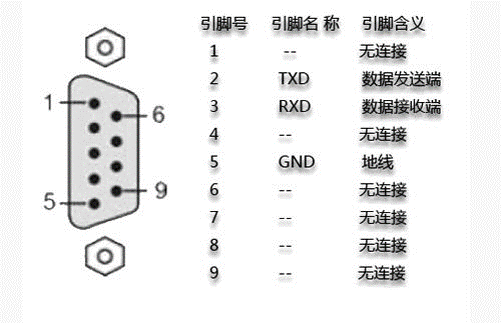
\includegraphics[width=0.5\textwidth]{img/3.PNG}
  \caption{相关原理图}
  \label{fig:3}
\end{figure}

MSP432 上包含了 8 个兼容不同通信协议的模块—4个 eUSCI\_A 和 4 个 eUSCI\_B。其中, eUSCI\_A 兼容 UART、 SPI。 eUSCI\_B 兼容 I2C、 SPI。在同一个模块固件下,一个模块可以支持多路串行通信。

\subsection{URAT 实验所需函数}

\begin{ccode}
  bool UART_initModule (uint32_t moduleInstance, 
          const eUSCI_UART_Config *config)
\end{ccode}

\begin{itemize}
  \item 功能描述:初始化UART模块
  \item 参数描述:moduleInstance  指定使用的UART模块
  \item config    UART配置结构体
\end{itemize}

UART 配置结构体

\begin{itemize}
  \item selectClockSource  选择时钟源
  \item clockPrescalar     写入波特率寄存器的数
  \item firstModReg     第一阶段的调整器
  \item secondModReg     第二阶段的调整器
  \item parity             校验位,可选择无校验位、奇校验或偶校验
  \item msborLsbFirst     控制发送/接收移位寄存器的方向,可选择 LSB 或 MSB
  \item numberofStopBits   停止位的位数,可选择一位或两位
  \item uartMode     选择 uart 模式
  \item overSampling     波特率产生方式
\end{itemize}

\begin{ccode}
  void UART_enableInterrupt (uint32_t moduleInstance,   uint_fast8_t mask)
\end{ccode}

\begin{itemize}
  \item 功能描述: 使能UART模块指定中断
  \item 参数描述:moduleInstance  指定使用的UART模块
  \item mask      指定中断类型
\end{itemize}

\section{实验步骤}

\subsection{URAT 实验}

\begin{itemize}
  \item 打开位于工程10\_01的uart工程;
  \item 点击编译并下载至LaunchPad开发板;
  \item 使用串口工具打开LaunchPad开发板XDS110 Class Application/User UART串口,串口配置参数:波特率为9600,8位数据位,无校验位,1位停止位,无流控;
  \item 在串口工具中发送任意单个ASCII字符,观察串口工具回显内容。
\end{itemize}

返回第一个字符的16进制ascii

\subsection{RTC实验}

\begin{itemize}
  \item 打开位于工程10\_02的rtc工程;
  \item 点击编译并下载至LaunchPad开发板;
  \item 使用串口工具打开LaunchPad开发板XDS110 Class Application/User UART串口,串口配置参数:波特率为9600,8位数据位,无校验位,1位停止位,无流控;
  \item 观察串口工具回显数据,说明实验现象。
\end{itemize}

\begin{figure}[h]
  \centering
  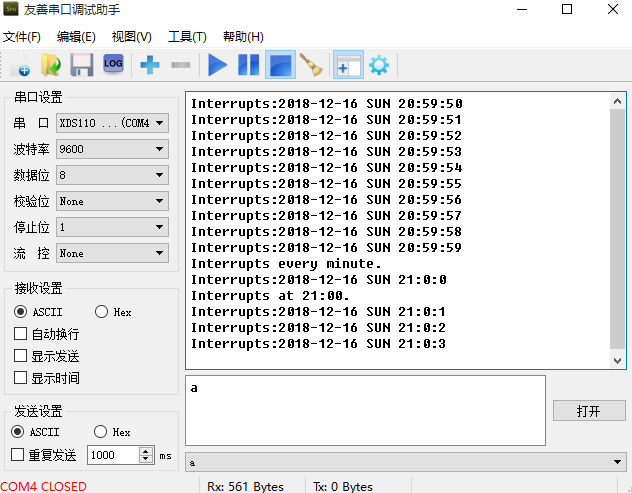
\includegraphics[width=0.5\textwidth]{img/4.PNG}
  \caption{实验结果}
  \label{fig:4}
\end{figure}

发现有三个中断事件,第一个每隔一秒发生第二个每分钟第三个每到21:00发生

\subsection{课堂练习}

\begin{itemize}
  \item 新建定时台灯keil工程,工程名为:light3\_学号,并保存到工程10\_03文件夹;
  \item 使用串口工具打开LaunchPad开发板XDS110 Class Application/User UART串口,串口配置参数:波特率为9600,8位数据位,无校验位,1位停止位,无流控;
  \item 在串口工具中发送数字“1”,则红灯被点亮;发送数字“2”,则绿灯被点亮;发送数字“3”,则蓝灯被点亮;发送其他ASCII字符,则RGB灯被熄灭。
\end{itemize}

思路:

\begin{itemize}
  \item 仿照实验一的路线,每次使用 UART 时引发中断
  \item 中断函数中通过 \texttt{MAP\_UART\_getEnabledInterruptStatus} 读取字符
  \item 如果字符是我们想要的,则改变 LED2 的颜色
  \item 否则关闭 LED2 
\end{itemize}

\section{调试过程、结果与分析}

每次urat发送中断读入一个字符判断他的ascii是否为0x31,0x32,0x33,然后在中断函数中通过gpio控制led

初始化 \texttt{GPIO LED2}

\begin{ccode}
  MAP_GPIO_setAsOutputPin(GPIO_PORT_P2, GPIO_PIN0);
  MAP_GPIO_setOutputLowOnPin(GPIO_PORT_P2, GPIO_PIN0);
  MAP_GPIO_setAsOutputPin(GPIO_PORT_P2, GPIO_PIN1);
  MAP_GPIO_setOutputLowOnPin(GPIO_PORT_P2, GPIO_PIN1);
  MAP_GPIO_setAsOutputPin(GPIO_PORT_P2, GPIO_PIN2);
  MAP_GPIO_setOutputLowOnPin(GPIO_PORT_P2, GPIO_PIN2);
\end{ccode}

配置urat

\begin{ccode}
  MAP_GPIO_setAsPeripheralModuleFunctionInputPin(GPIO_PORT_P1,GPIO_PIN2 
  | GPIO_PIN3, GPIO_PRIMARY_MODULE_FUNCTION);
  
  MAP_UART_initModule(EUSCI_A0_BASE, &uartConfig);

  MAP_UART_enableModule(EUSCI_A0_BASE);
  
  MAP_UART_enableInterrupt(EUSCI_A0_BASE, EUSCI_A_UART_RECEIVE_INTERRUPT);
  MAP_Interrupt_enableInterrupt(INT_EUSCIA0);  
  MAP_Interrupt_enableMaster();    
\end{ccode}

中断函数,\texttt{MAP\_UART\_receiveData(EUSCI\_A0\_BASE)} 会读入一个字符并且返回 ASCII 值,可以根据其是否为 0x31, 0x32, 0x33 来控制 LED2

\begin{ccode}
  void EUSCIA0_IRQHandler(void)
  {
    char tmp[3]={'\0'};
    uint32_t status = MAP_UART_getEnabledInterruptStatus(EUSCI_A0_BASE);
    if(status & EUSCI_A_UART_RECEIVE_INTERRUPT_FLAG)
    {          
      sprintf(tmp,"%x",MAP_UART_receiveData(EUSCI_A0_BASE));

      GPIO_setOutputLowOnPin(GPIO_PORT_P2, GPIO_PIN0);
      GPIO_setOutputLowOnPin(GPIO_PORT_P2, GPIO_PIN1);
      GPIO_setOutputLowOnPin(GPIO_PORT_P2, GPIO_PIN2);

      if (strcmp(tmp, "31") == 0) {
        GPIO_setOutputHighOnPin(GPIO_PORT_P2, GPIO_PIN0);
      } else if (strcmp(tmp, "32") == 0) {
        GPIO_setOutputHighOnPin(GPIO_PORT_P2, GPIO_PIN1);
      } else if (strcmp(tmp, "33") == 0) {
        GPIO_setOutputHighOnPin(GPIO_PORT_P2, GPIO_PIN2);
      }
    }   
  }
\end{ccode}

\section{总结}

\begin{itemize}
  \item 之前的中断函数大多需要清空中断标志,但是 UART 不用
  \item UART 输入得到的结果是 ASCII 码,如果需要转换成对应的数字需要做相应的计算
  \item 串口调试工具可以使用清空内容来清理输入输出框
\end{itemize}
  
\section{附件}

\end{document}
